\documentclass[class=article, crop=false]{standalone}
\usepackage[margin=1in]{geometry}
\usepackage[linesnumbered,ruled,vlined]{algorithm2e}
\usepackage{amsfonts}
\usepackage{amsmath}
\usepackage{amssymb}
\usepackage{amsthm}
\usepackage{enumitem}
\usepackage{fancyhdr}
\usepackage{hyperref}
\usepackage{minted}
\usepackage{multicol}
\usepackage{pdfpages}
\usepackage{standalone}
\usepackage[many]{tcolorbox}
\usepackage{tikz-cd}
\usepackage{transparent}
\usepackage{xcolor}
% \tcbuselibrary{minted}

\author{Nathan Solomon}

\newcommand{\fig}[1]{
    \begin{center}
        \includegraphics[width=\textwidth]{#1}
    \end{center}
}

% Math commands
\renewcommand{\d}{\mathrm{d}}
\DeclareMathOperator{\id}{id}
\DeclareMathOperator{\im}{im}
\DeclareMathOperator{\proj}{proj}
\DeclareMathOperator{\Span}{span}
\DeclareMathOperator{\Tr}{Tr}
\DeclareMathOperator{\tr}{tr}
\DeclareMathOperator{\ad}{ad}
\DeclareMathOperator{\ord}{ord}
%%%%%%%%%%%%%%% \DeclareMathOperator{\sgn}{sgn}
\DeclareMathOperator{\Aut}{Aut}
\DeclareMathOperator{\Inn}{Inn}
\DeclareMathOperator{\Out}{Out}
\DeclareMathOperator{\stab}{stab}

\newcommand{\N}{\ensuremath{\mathbb{N}}}
\newcommand{\Z}{\ensuremath{\mathbb{Z}}}
\newcommand{\Q}{\ensuremath{\mathbb{Q}}}
\newcommand{\R}{\ensuremath{\mathbb{R}}}
\newcommand{\C}{\ensuremath{\mathbb{C}}}
\renewcommand{\H}{\ensuremath{\mathbb{H}}}
\newcommand{\F}{\ensuremath{\mathbb{F}}}

\newcommand{\E}{\ensuremath{\mathbb{E}}}
\renewcommand{\P}{\ensuremath{\mathbb{P}}}

\newcommand{\es}{\ensuremath{\varnothing}}
\newcommand{\inv}{\ensuremath{^{-1}}}
\newcommand{\eps}{\ensuremath{\varepsilon}}
\newcommand{\del}{\ensuremath{\partial}}
\renewcommand{\a}{\ensuremath{\alpha}}

\newcommand{\abs}[1]{\ensuremath{\left\lvert #1 \right\rvert}}
\newcommand{\norm}[1]{\ensuremath{\left\lVert #1\right\rVert}}
\newcommand{\mean}[1]{\ensuremath{\left\langle #1 \right\rangle}}
\newcommand{\floor}[1]{\ensuremath{\left\lfloor #1 \right\rfloor}}
\newcommand{\ceil}[1]{\ensuremath{\left\lceil #1 \right\rceil}}
\newcommand{\bra}[1]{\ensuremath{\left\langle #1 \right\rvert}}
\newcommand{\ket}[1]{\ensuremath{\left\lvert #1 \right\rangle}}
\newcommand{\braket}[2]{\ensuremath{\left.\left\langle #1\right\vert #2 \right\rangle}}

\newcommand{\catname}[1]{{\normalfont\textbf{#1}}}

\newcommand{\up}{\ensuremath{\uparrow}}
\newcommand{\down}{\ensuremath{\downarrow}}

% Custom environments
\newtheorem{thm}{Theorem}[section]

\definecolor{probBackgroundColor}{RGB}{250,240,240}
\definecolor{probAccentColor}{RGB}{140,40,0}
\newenvironment{prob}{
    \stepcounter{thm}
    \begin{tcolorbox}[
        boxrule=1pt,
        sharp corners,
        colback=probBackgroundColor,
        colframe=probAccentColor,
        borderline west={4pt}{0pt}{probAccentColor},
        breakable
    ]
    \color{probAccentColor}\textbf{Problem \thethm.} \color{black}
} {
    \end{tcolorbox}
}

\definecolor{exampleBackgroundColor}{RGB}{212,232,246}
\newenvironment{example}{
    \stepcounter{thm}
    \begin{tcolorbox}[
      boxrule=1pt,
      sharp corners,
      colback=exampleBackgroundColor,
      breakable
    ]
    \textbf{Example \thethm.}
} {
    \end{tcolorbox}
}

\definecolor{propBackgroundColor}{RGB}{255,245,220}
\definecolor{propAccentColor}{RGB}{150,100,0}
\newenvironment{prop}{
    \stepcounter{thm}
    \begin{tcolorbox}[
        boxrule=1pt,
        sharp corners,
        colback=propBackgroundColor,
        colframe=propAccentColor,
        breakable
    ]
    \color{propAccentColor}\textbf{Proposition \thethm. }\color{black}
} {
    \end{tcolorbox}
}

\definecolor{thmBackgroundColor}{RGB}{235,225,245}
\definecolor{thmAccentColor}{RGB}{50,0,100}
\renewenvironment{thm}{
    \stepcounter{thm}
    \begin{tcolorbox}[
        boxrule=1pt,
        sharp corners,
        colback=thmBackgroundColor,
        colframe=thmAccentColor,
        breakable
    ]
    \color{thmAccentColor}\textbf{Theorem \thethm. }\color{black}
} {
    \end{tcolorbox}
}

\definecolor{corBackgroundColor}{RGB}{240,250,250}
\definecolor{corAccentColor}{RGB}{50,100,100}
\newenvironment{cor}{
    \stepcounter{thm}
    \begin{tcolorbox}[
        enhanced,
        boxrule=0pt,
        frame hidden,
        sharp corners,
        colback=corBackgroundColor,
        borderline west={4pt}{0pt}{corAccentColor},
        breakable
    ]
    \color{corAccentColor}\textbf{Corollary \thethm. }\color{black}
} {
    \end{tcolorbox}
}

\definecolor{lemBackgroundColor}{RGB}{255,245,235}
\definecolor{lemAccentColor}{RGB}{250,125,0}
\newenvironment{lem}{
    \stepcounter{thm}
    \begin{tcolorbox}[
        enhanced,
        boxrule=0pt,
        frame hidden,
        sharp corners,
        colback=lemBackgroundColor,
        borderline west={4pt}{0pt}{lemAccentColor},
        breakable
    ]
    \color{lemAccentColor}\textbf{Lemma \thethm. }\color{black}
} {
    \end{tcolorbox}
}

\definecolor{proofBackgroundColor}{RGB}{255,255,255}
\definecolor{proofAccentColor}{RGB}{80,80,80}
\renewenvironment{proof}{
    \begin{tcolorbox}[
        enhanced,
        boxrule=1pt,
        sharp corners,
        colback=proofBackgroundColor,
        colframe=proofAccentColor,
        borderline west={4pt}{0pt}{proofAccentColor},
        breakable
    ]
    \color{proofAccentColor}\emph{\textbf{Proof. }}\color{black}
} {
    \qed \end{tcolorbox}
}

\definecolor{noteBackgroundColor}{RGB}{240,250,240}
\definecolor{noteAccentColor}{RGB}{30,130,30}
\newenvironment{note}{
    \begin{tcolorbox}[
        enhanced,
        boxrule=0pt,
        frame hidden,
        sharp corners,
        colback=noteBackgroundColor,
        borderline west={4pt}{0pt}{noteAccentColor},
        breakable
    ]
    \color{noteAccentColor}\textbf{Note. }\color{black}
} {
    \end{tcolorbox}
}



\fancyhf{}
\lhead{Nathan Solomon}
\rhead{Page \thepage}
\pagestyle{fancy}

\begin{document}
\section{The Catholic Baroque}
The Byzantine Empire fell in 1453, and after that, the Catholic church gained a lot of power. They took advantage of ``indulgences" (donations to the church in order to absolve your sins so you are more likely to get into Heaven) in order to raise money for fancy buildings.
\par
Just like with Ninomaru Palace, the large Baroque buildings built by Catholics were used to demonstrate authority and strength. They often take a long time to build though, like the Saint Peter's Basilica in Vatican City (1506-1626). Because of that, the styles change during the time it's being built.
\par
Previously, buildings were made by guilds members and other laborors, but Saint Peter's Basilica was one of the first large projects to be led by architects who had a clear vision, but even still, the final product was very different from the initial plan. Initially, they planned to use a ``Greek cross", then started trying to use a ``Latin cross" instead, and then extended the entrance even more.
\par
One influential building from a similar time was the protestant church in Westerkerk, Amsterdam, called the Hendrick de Keyser (1620-1631). It used exposed brick, dark brown, relatively simple arches, and no stained glass. It still looks pretty fancy, but by the standards for churches at the time, it was considered very muted and humble. This challenged the authority of the catholic church.
\par
The catholic church's response was to develop the Baroque style. It wasn't just an architectural style, but also included styles of music and fashion that became part of the counter-reformation.
\par
\textbf{Baroquism} is a 17th and 18th century stylistic movement in art, musc, and architecture, characterized by elaborate and highly expressive ornamentation.
\par
The modern motto used to describe the philosphy of Baroquism is ``more is more". Baroque buildings were extremely ornate and detailed to the point of feeling cluttered. On the inside, they were even more ornate and colorful, with paintings and gold all over the ceilings.
\par
Baroque churches began to include large plazzas which emphasized the scale/importance of the church, and the plazzas were also practical for events with lots of people. In terms of urban design, this was sort of a revival of Roman styles. In the Baroque period, people also began using a street layout called \textbf{trivium}, which features 3 straight roads converging on a single building or open space. City planning demonstrates that there is a central authority, who can command for entire streets to be demolished and rebuilt.
\par
As with any architectural movement, once the rules are established, people are eager to break them. For example, the Church of San Carlo alle Quattro Fontane (1638-1646( in Rome, shown below, distorted the roofs and arches that were typically used in Baroque buildings.
\begin{center}
    \includegraphics[width=\textwidth]{San_Carlo_alle_Quattro_Fontane_-_Front.jpg}
\end{center}
Meanwhile, in Spain, the ``reconquista" (722-1492) was the military reconquering of Muslims by Christians. Because of the mixing of cultures, the newly formed Spanish empire was heavily influenced by Muslim architecture, which they brought to the Americas. In 1521, Spanish colonizers defeated the Aztecs in Tenochtitlán. Tenochtitlán was built on an elegant grid system with aqueducts and other nice infrastructure, which the Spaniards liked, but they tore down the old temples and built Mexico City on the ruins, while keeping the overall structue, as well as some of the buildings and infrastructure.
\par
The \textbf{Laws of the Indies} were a series of 150 Spanish ordinances that dictated the layout of their colonial cities. Notably, they were required to use a rectangular grid with a central plaza called the \textit{plaza mayor}. Despite saying they were ``civilizing" the ``savages", many of those ideas were taken from the natives and rebranded as a uniquely Spanish style.
\par
\textbf{Mestizo Baroque} is an umbrella term for various hybrids of Baroque European and indigenous arts and architectures found throughout the Spanish colonial Americas. It developed much later than the Baroque style in Europe, because of the physical distance from Europe, weaker economy (than Europe), and reluctant workforce.
\par
A famous example of the Mestize Baroque style is the San Lorenzo de Carangas, in Potosí, Bolivia (1548-1744), shown below.
\begin{center}
    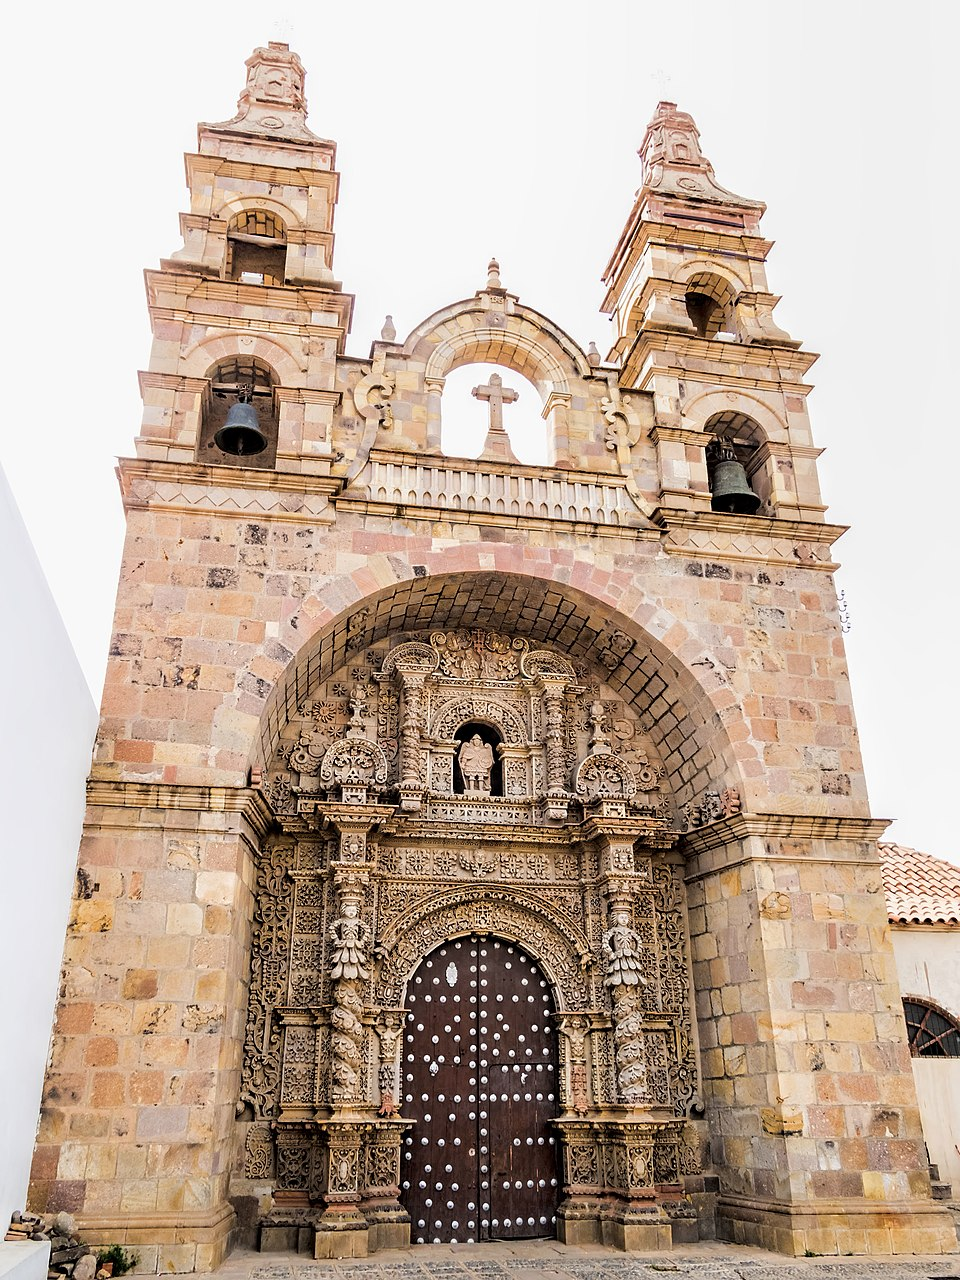
\includegraphics[width=\textwidth]{San Lorenzo de Carangas.jpg}
\end{center}


\end{document}
